\question{Câu 5}

Cho mạch khuếch đại tín hiệu được ghép liên tầng như hình vẽ. Trong đó, $Q_{1}$ là BJT có $\beta = 100$ và mã 2SC1815, và $Q_{2}$ có $\beta = 80$ có mã là 2N2907.

\begin{figure}[H]
	\centering
	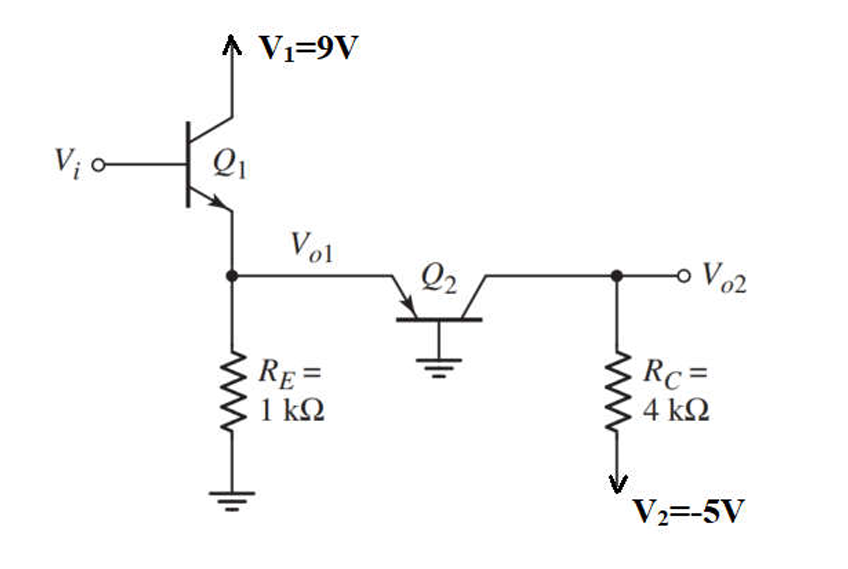
\includegraphics[width=.8\linewidth]{./my-chapters/my-images/Question5/debai.png}
\end{figure}

\answer{a}{Sử dụng phần mềm mô phỏng, vẽ VTC của mạch (ngõ vào $V_{i}$ và ngõ ra là $V_{o}$).}

Sử dụng chế độ DC Sweep trong Multisim để khảo sát VTC,

\begin{figure}[H]
	\centering
	\begin{minipage}{.5\linewidth}
		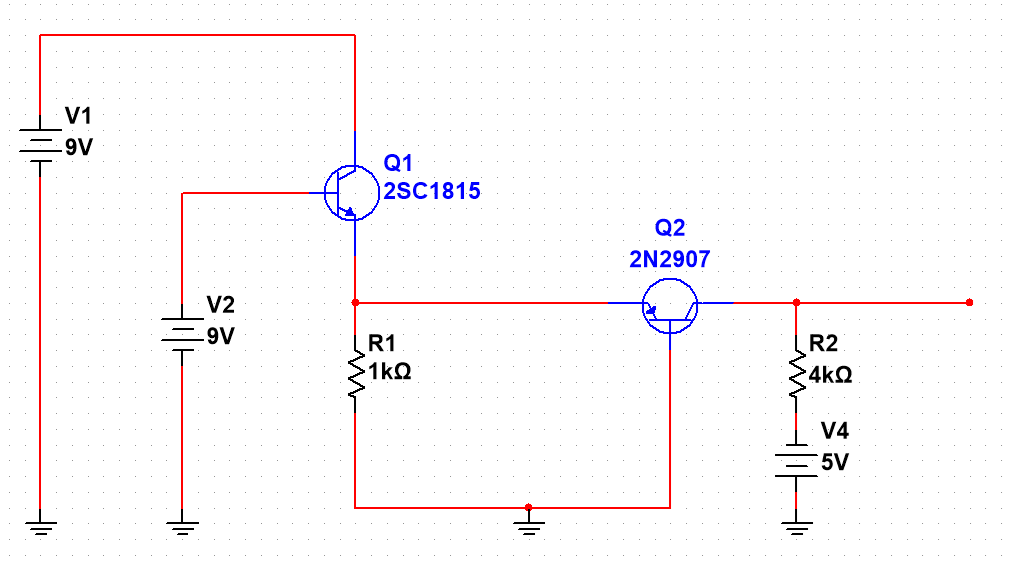
\includegraphics[width=.8\linewidth]{./my-chapters/my-images/Question5/a_mach.png}
	\end{minipage}
	\begin{minipage}{.4\linewidth}
		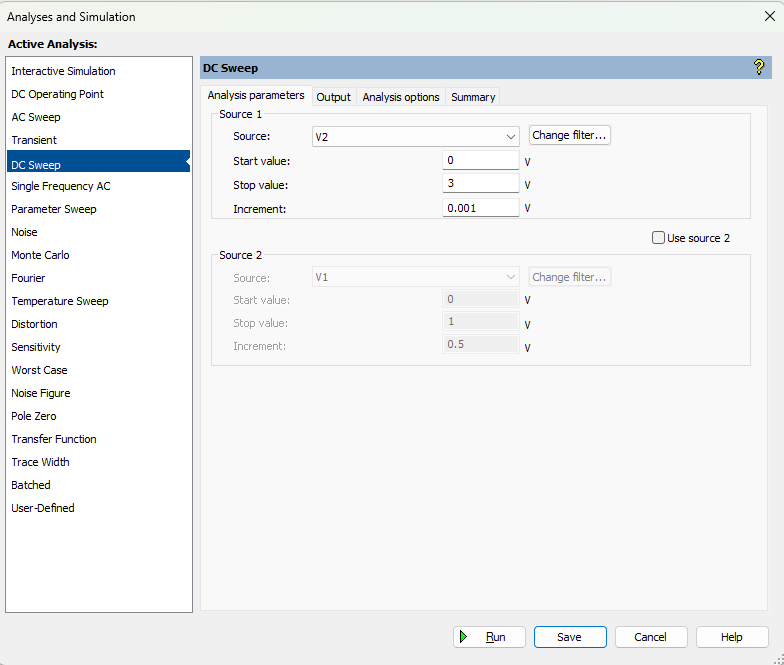
\includegraphics[width=.8\linewidth]{./my-chapters/my-images/Question5/a_dc_sweep.png}
	\end{minipage}
\end{figure}

\begin{figure}[H]
	\centering
	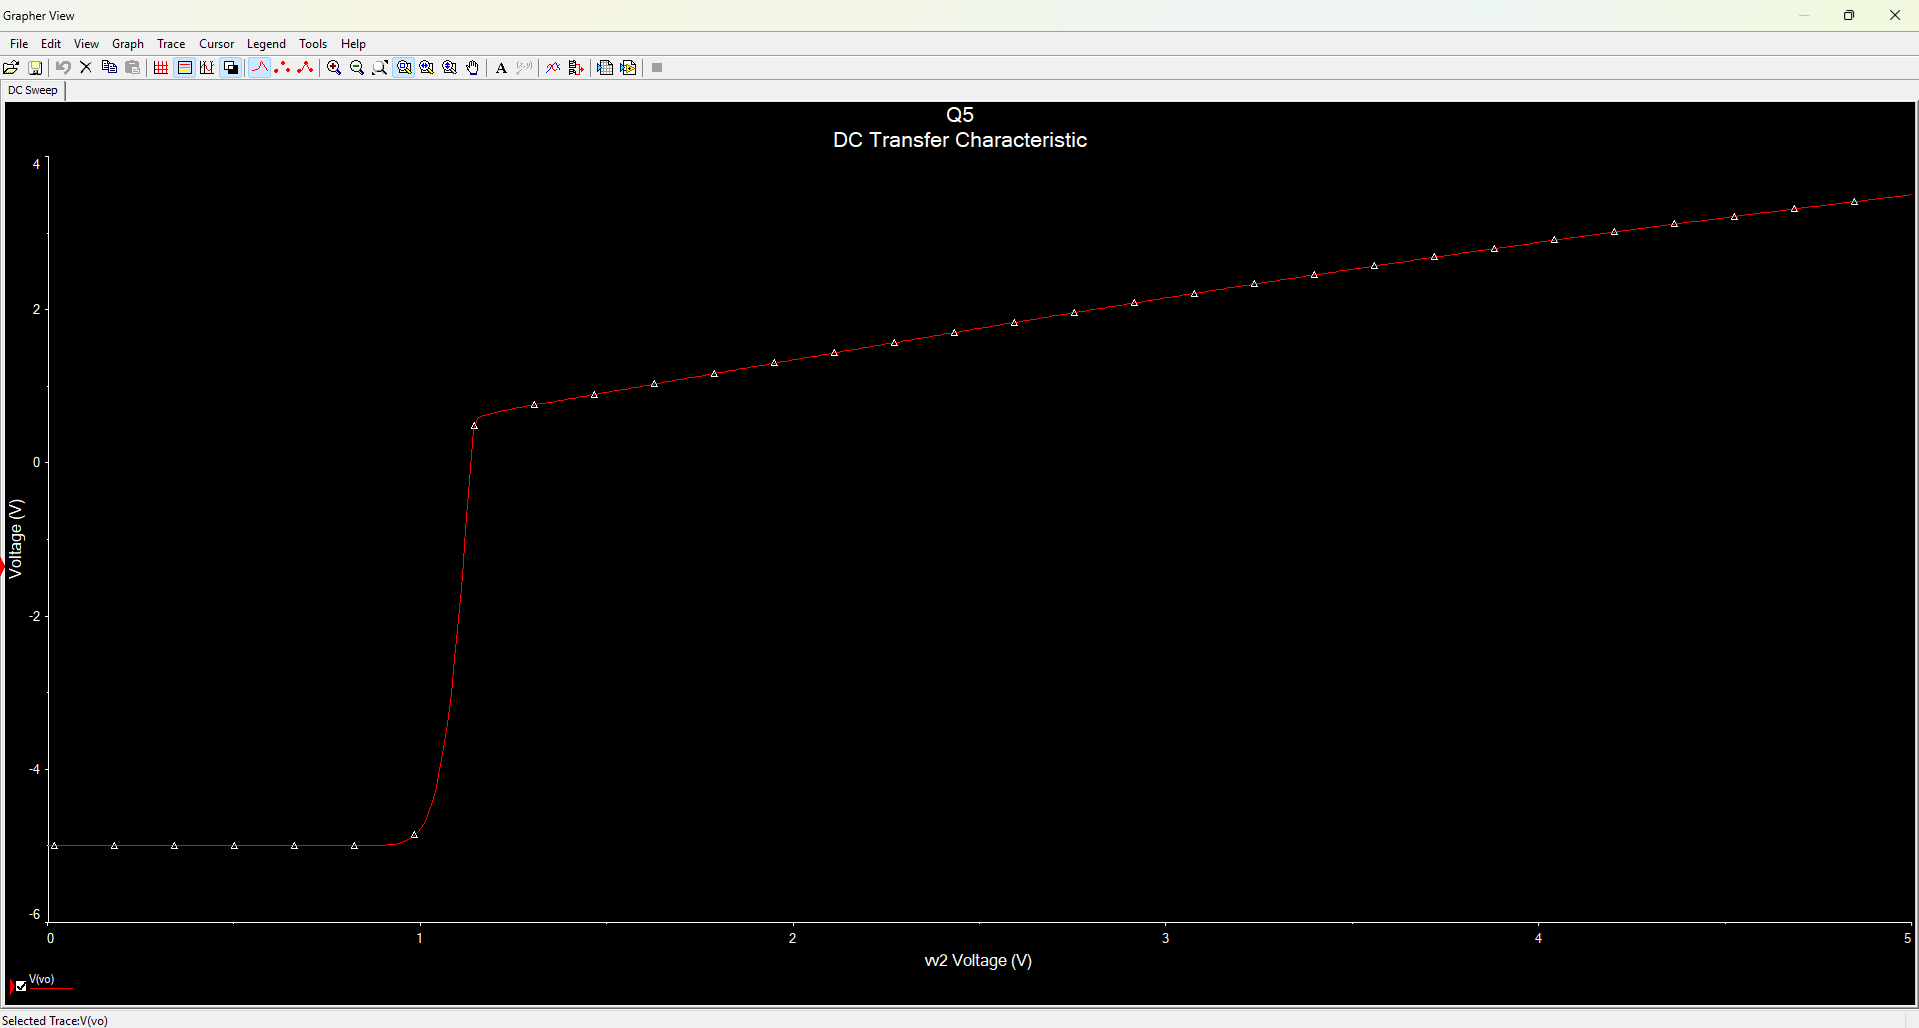
\includegraphics[width=.9\linewidth]{./my-chapters/my-images/Question5/a_VTC.png}
	\caption{VTC của mạch với ngõ vào $V_{i}$ và ngõ ra là $V_{o}$.}
\end{figure}

\begin{minipage}{0.4\linewidth}
	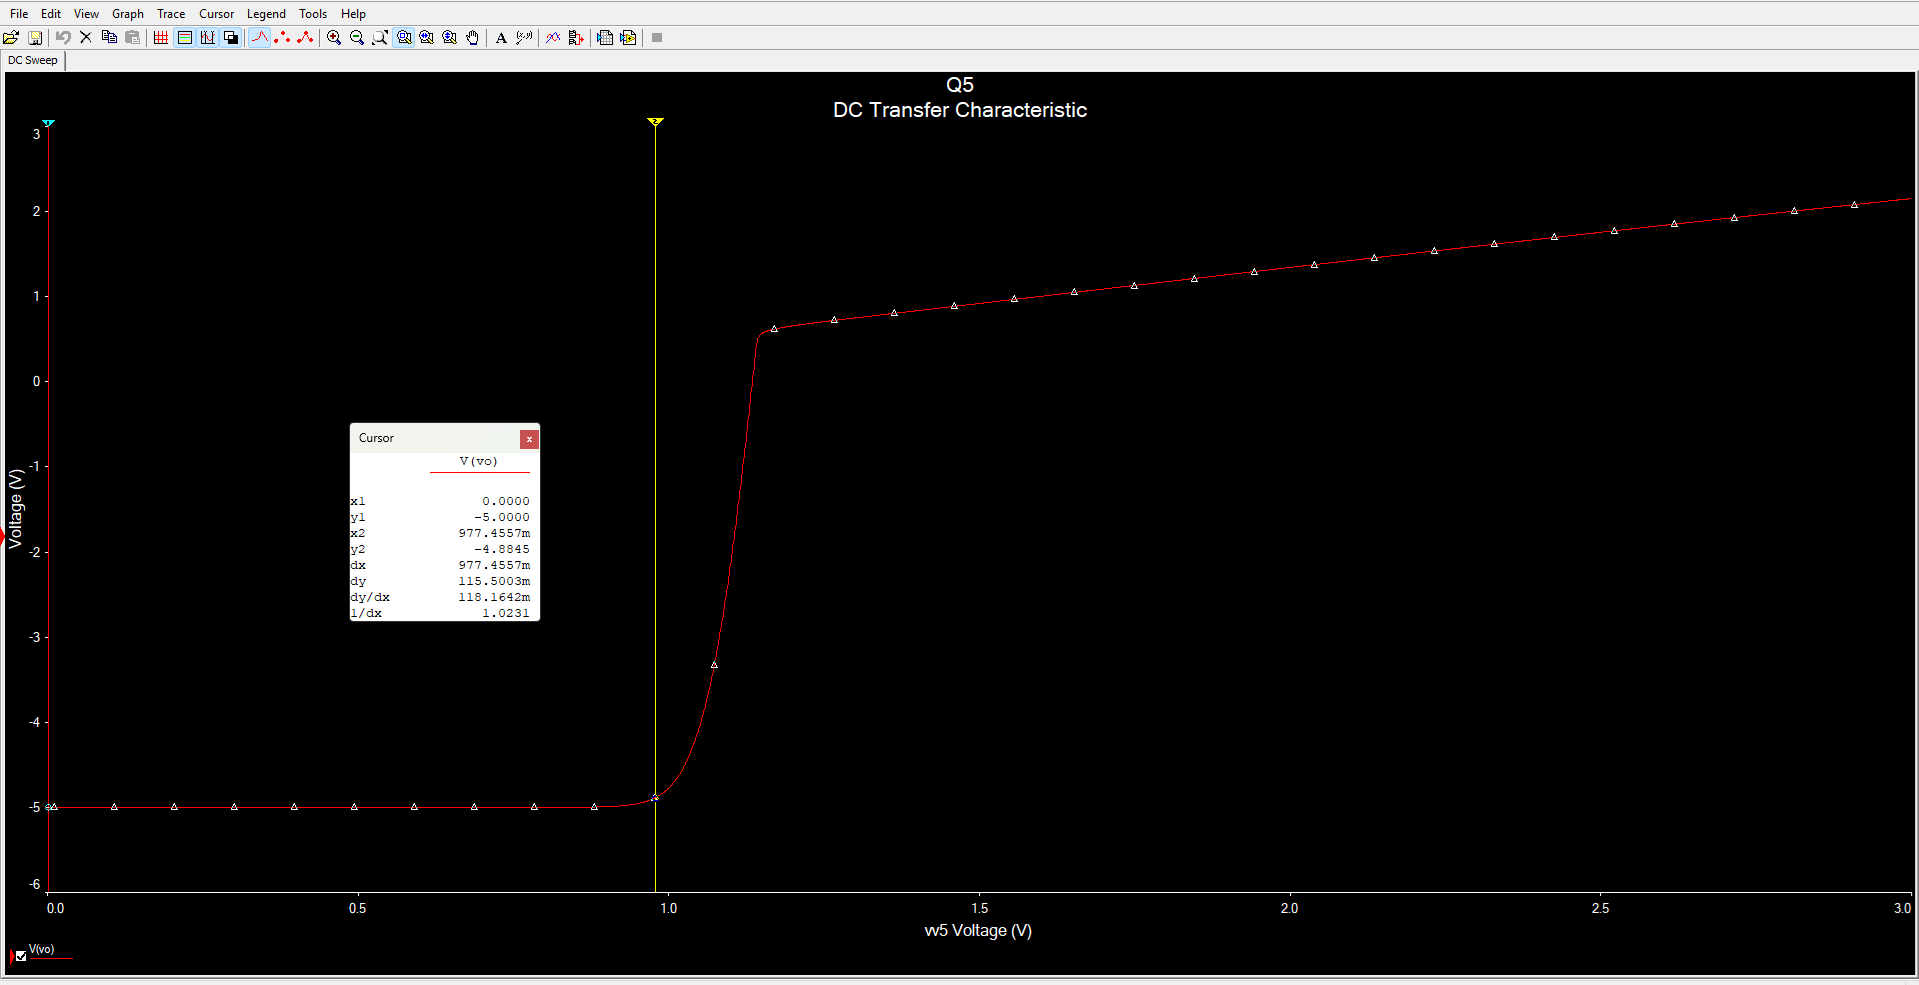
\includegraphics[width=\linewidth]{./my-chapters/my-images/Question5/a_cutoff.png}
\end{minipage}
\begin{minipage}{0.5\linewidth}
	\begin{itemize}[label=-]
		\item Với $V_{i} < 0.9775\,\textsf{V}$ thì mạch bị rơi vào miền cut off, lúc này ngõ ra của mạch luôn bằng $V_{EE} = -5\,\textsf{V}$.
		
		\item Với $0.9775 < V_{i} < 1.1675\,\textsf{V}$ thì mạch trong miền khuếch đại, với độ dốc lớn.
	\end{itemize}
\end{minipage}

\begin{minipage}{0.4\linewidth}
	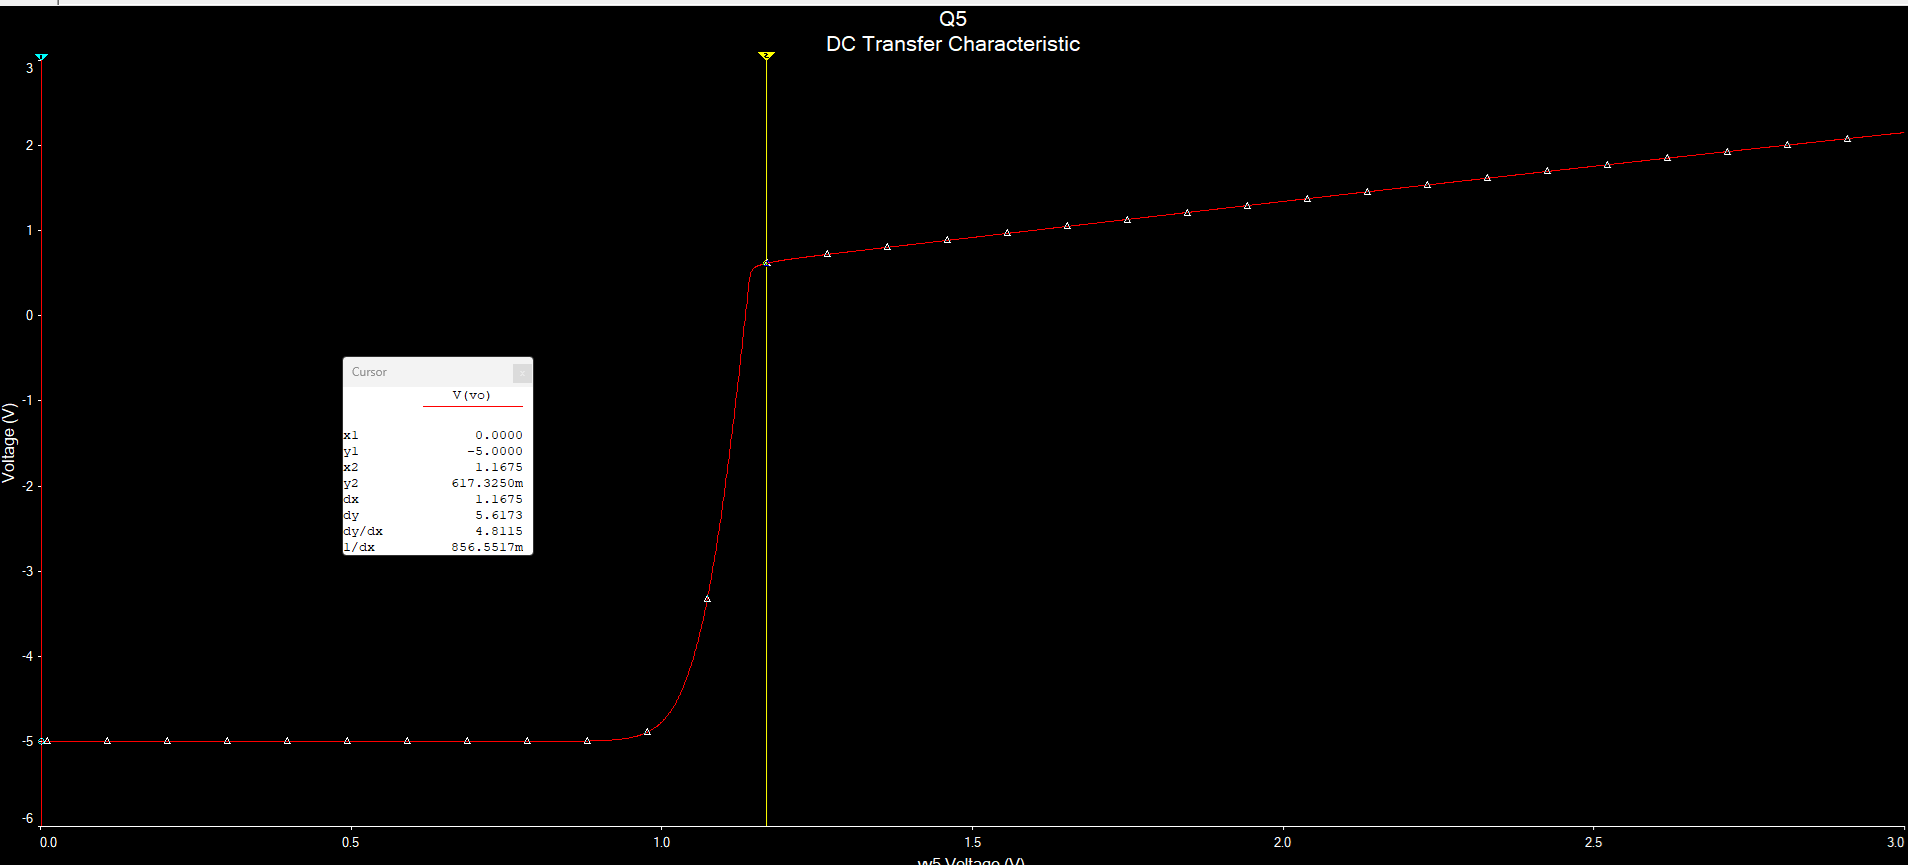
\includegraphics[width=\linewidth]{./my-chapters/my-images/Question5/a_linear.png}
\end{minipage}
\begin{minipage}{0.5\linewidth}
	\begin{itemize}[label=-]
		\item Với $V_{i} > 1.1675\,\textsf{V}$ thì mạch trong miền bão hòa.
	\end{itemize}
\end{minipage}
\answer{b}{Lựa chọn điểm phân cực của cả mạch trên VTC và thiết kế mạch ghép vào phía trước VTC để có được điểm phân cực đó.}

Quan sát VTC của mạch, để tín hiệu ngõ ra không bị méo dạng thì ta chọn điểm $Q$ với $V_{i} = 1.0998\,\text{V}$.

\begin{figure}[H]
	\centering
	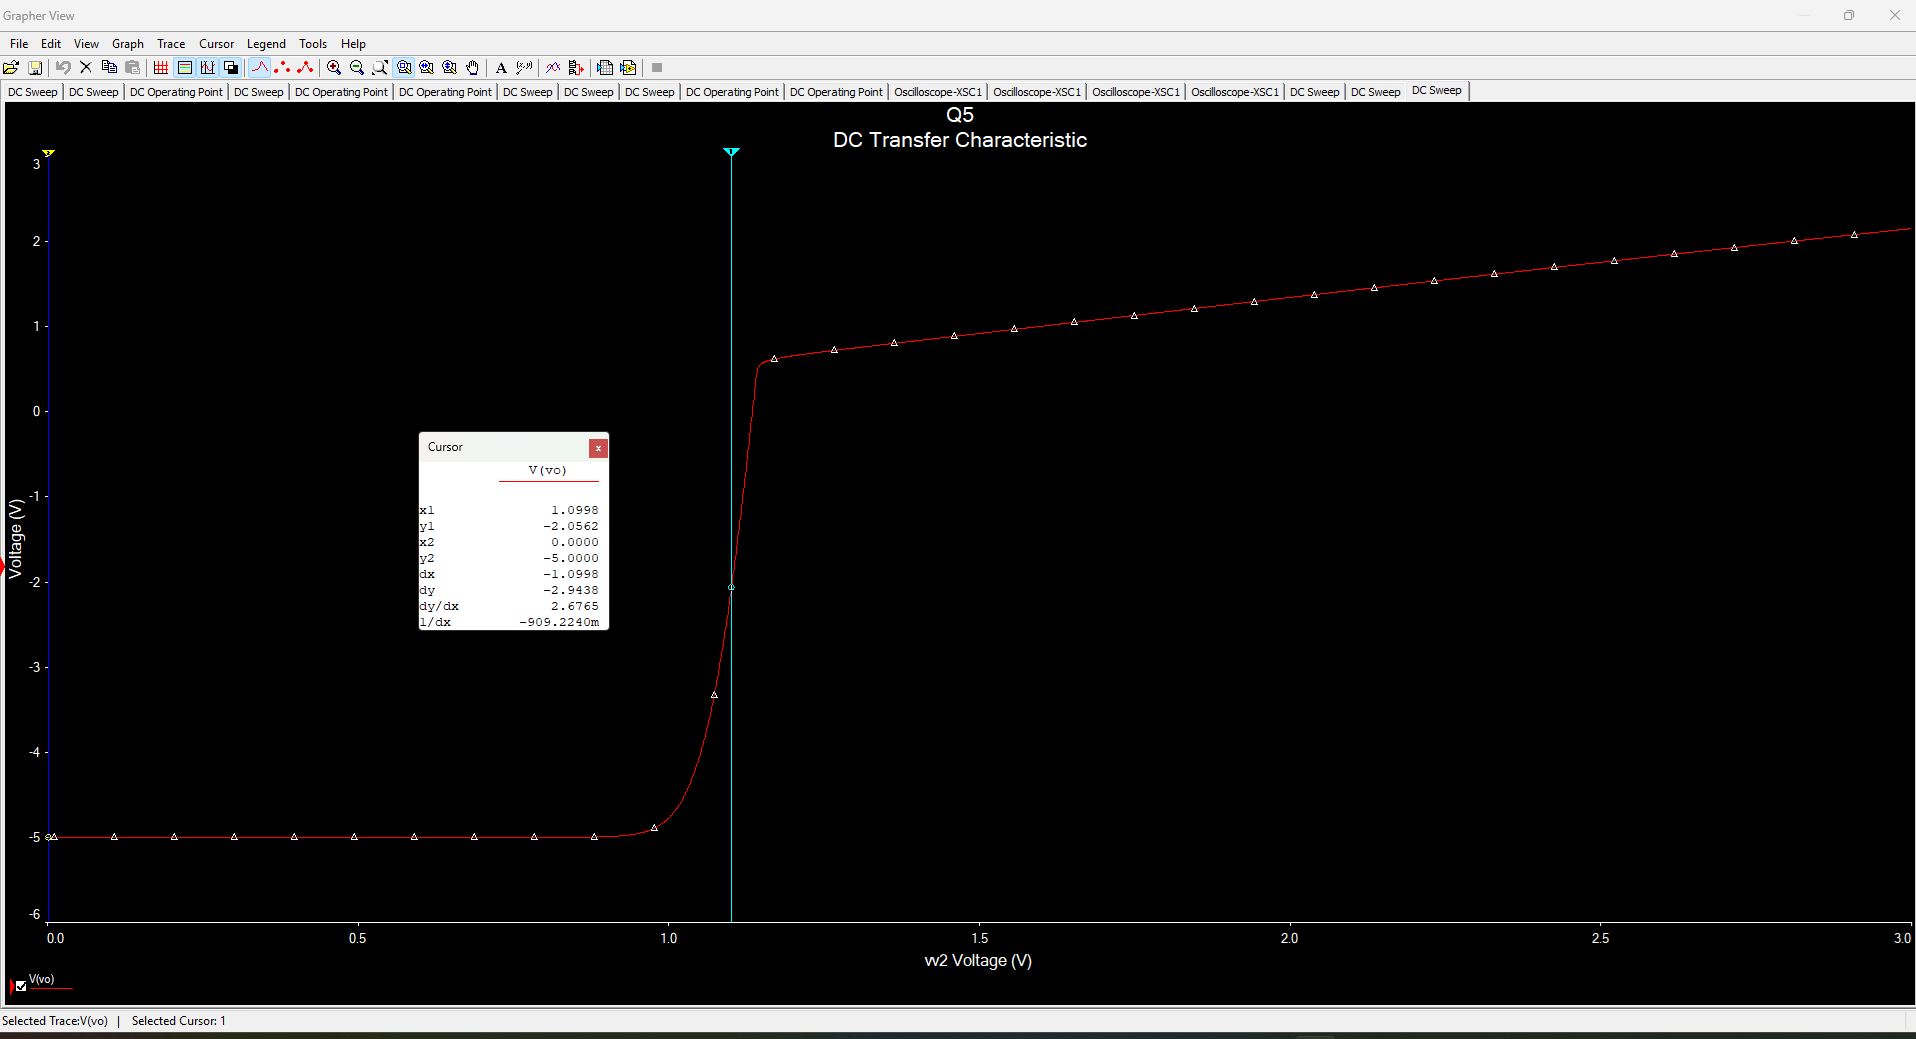
\includegraphics[width=.9\linewidth]{./my-chapters/my-images/Question5/b_Q_tong.png}
	\caption{Điểm hoạt động của toàn mạch rơi vào tầm $V_{i} = 1.0998\,\text{V}$ để tín hiệu $V_{o}$ không méo dạng.}
\end{figure}

Với $V_{i} = 1.0998\,\text{V}$, ta chọn được hai điểm:

\begin{figure}[H]
	\centering
%	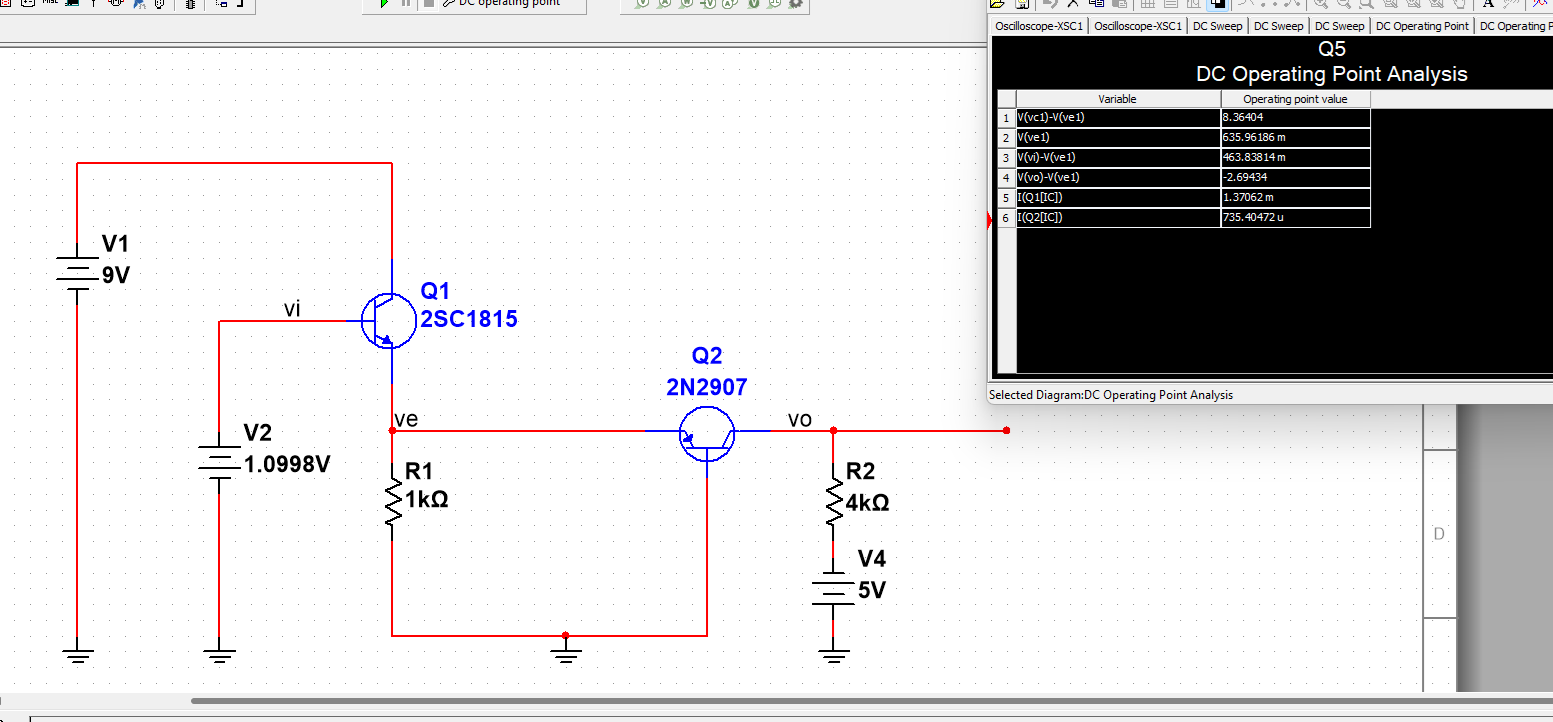
\includegraphics[width=.9\linewidth]{./my-chapters/my-images/Question5/b_Q_tung_mach.png}
	\begin{minipage}{.4\linewidth}
		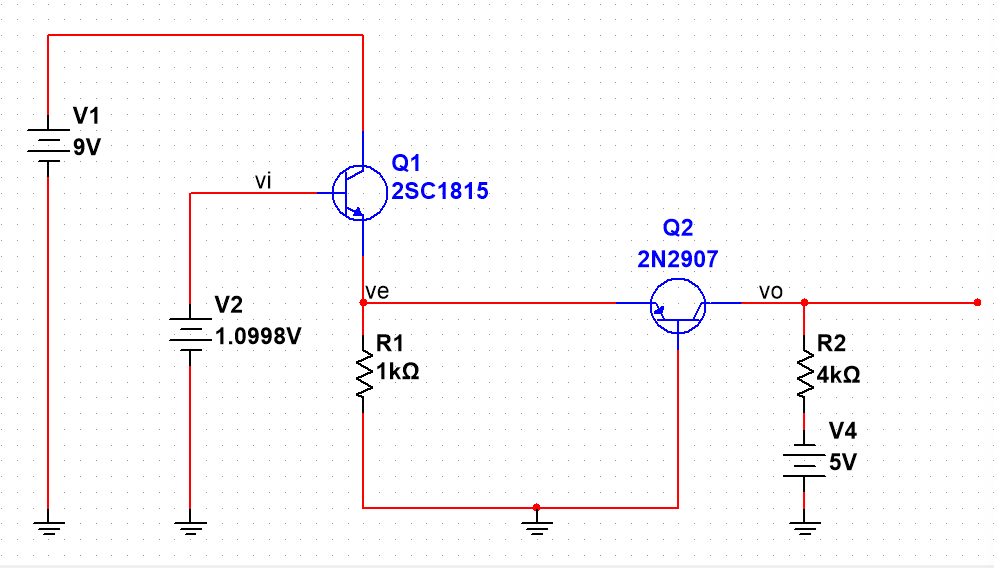
\includegraphics[width=\linewidth]{./my-chapters/my-images/Question5/b_Q_tong_hinh.png}
	\end{minipage}
	\begin{minipage}{.5\linewidth}
		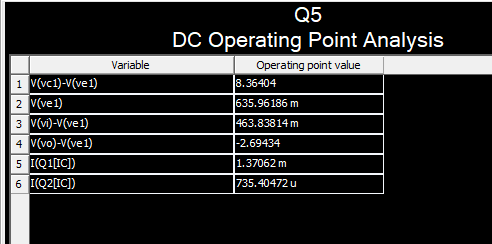
\includegraphics[width=\linewidth]{./my-chapters/my-images/Question5/b_Q_tong_bang.png}
	\end{minipage}
\end{figure}

\begin{itemize}[label=-, leftmargin=2cm]
	\item \finalresult{Q_{1} = (I_{CQ1}, V_{CEQ1}) = (1.3706\,\text{mA}, 8.3640\,\text{V})}
	\item \finalresult{Q_{2} = (I_{CQ2}, V_{CEQ2}) = (0.7354\,\text{mA}, -2.6943\,\text{V})}
\end{itemize}

Ta sử dụng một mạch phân cực $R_{1}$ và $R_{2}$ như sau:

\begin{figure}[H]
	\centering
	\begin{minipage}{.4\linewidth}
		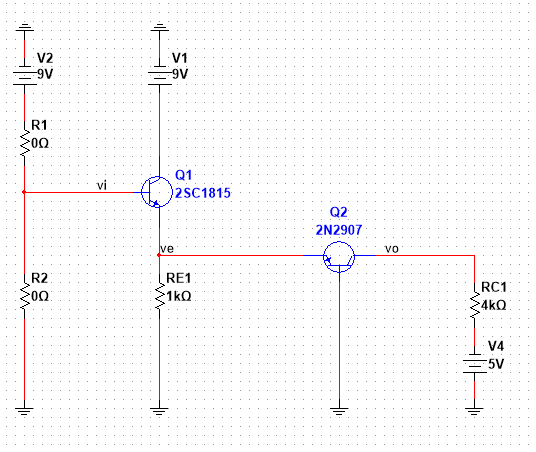
\includegraphics[width=\linewidth]{./my-chapters/my-images/Question5/b_phancuc_R1_R2.png}
	\end{minipage}
	\begin{minipage}{.1\linewidth}
		$\Rightarrow$
	\end{minipage}
	\begin{minipage}{.4\linewidth}
		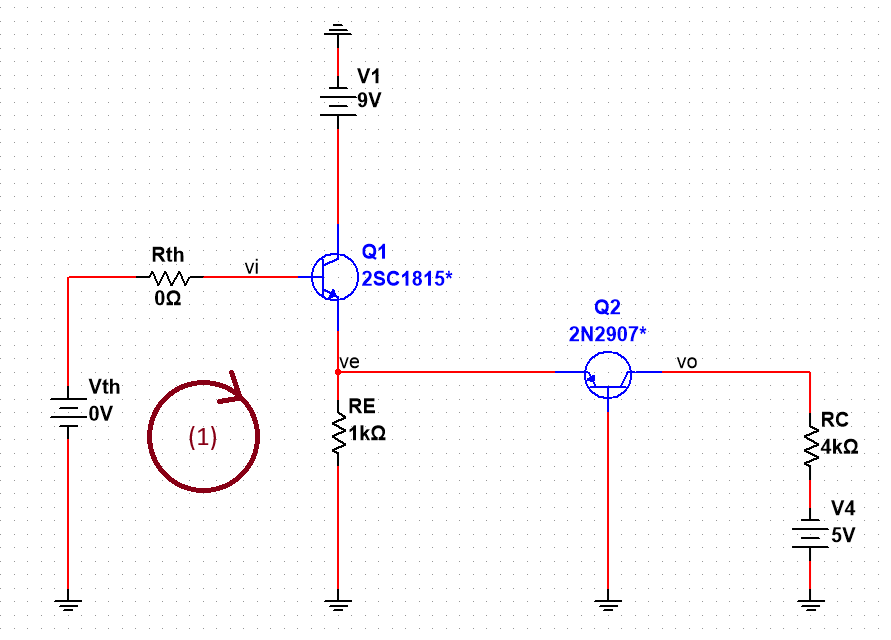
\includegraphics[width=\linewidth]{./my-chapters/my-images/Question5/b_phancuc_thevenin.png}
	\end{minipage}
\end{figure}

Ta có, $I_{C1} = 1.3706\,\text{mA} \Rightarrow I_{B1} = \dfrac{I_{C1}}{\beta} = \dfrac{1.3706}{100} = 0.013706\,\text{mA}$.

$I_{RE} = I_{E1} - I_{E2} = \dfrac{I_{C1}}{\alpha} - \dfrac{I_{C2}}{\alpha} = \dfrac{1.3706}{\dfrac{100}{100+1}} - \dfrac{0.7354}{\dfrac{100}{100+1}} = 0.64582\,\text{mA}$

Viết KCL cho vòng (1):

\[ V_{th} = R_{th}I_{B1} + V_{BE1} + I_{RE}R_{E} \]
\[ \Leftrightarrow 9\times \dfrac{R_{2}}{R_{1} + R_{2}} = \dfrac{R_{1}R_{2}}{R_{1} + R_{2}}\times I_{B1} + V_{BE1} + R_{E}I_{RE} \]
\[ \Leftrightarrow \dfrac{R_{2}}{R_{1} + R_{2}}\left( 9 - R_{1}\times 0.013706 \right) = 1.1097 \]

Với chọn $R_{2} = 22\,\text{k}\Omega \Rightarrow R_{1} = 123.0036\,\text{k}\Omega$.

Kết quả mô phỏng,

\begin{figure}[H]
	\centering
	\begin{minipage}{.4\linewidth}
		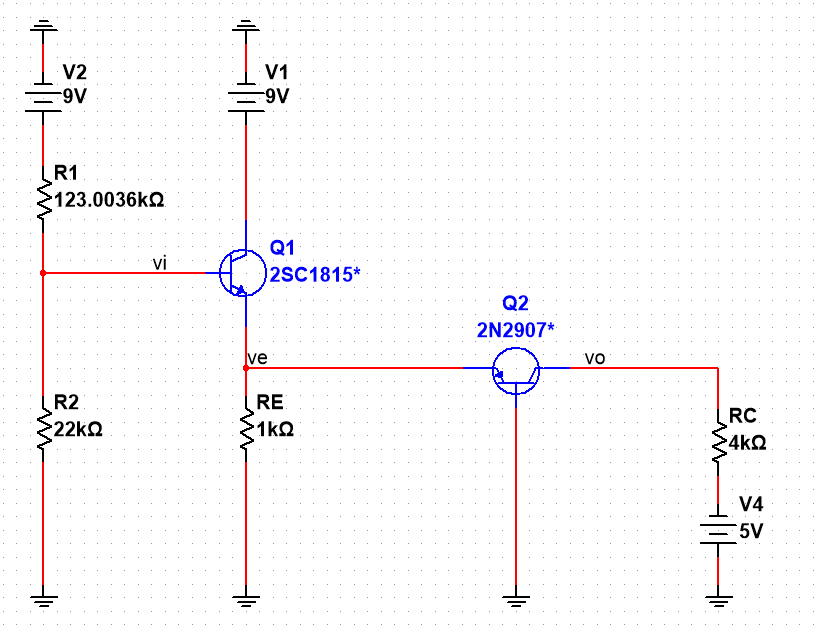
\includegraphics[width=\linewidth]{./my-chapters/my-images/Question5/b_ketqua_R1R2.png}
	\end{minipage}
	\begin{minipage}{.4\linewidth}
		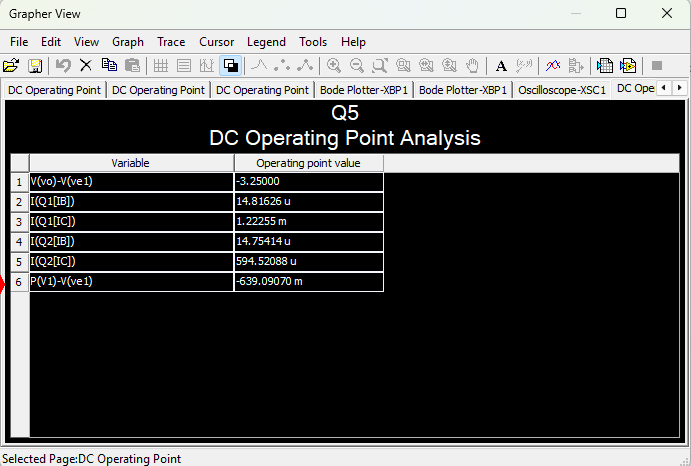
\includegraphics[width=\linewidth]{./my-chapters/my-images/Question5/b_ketqua.png}
	\end{minipage}
\end{figure}

\answer{c}{Lựa chọn tụ $C_{1}$ (ghép tín hiệu) và $C_{2}$ (ghép tải) để mạch có $f_{L}=200Hz$. Giả sử tín hiệu có nội trở $100\Omega$ và tải có điện trở $100\Omega$. Sử dụng phần mềm mô phỏng, vẽ đáp ứng tần số của mạch.}

\begin{figure}[H]
	\centering
	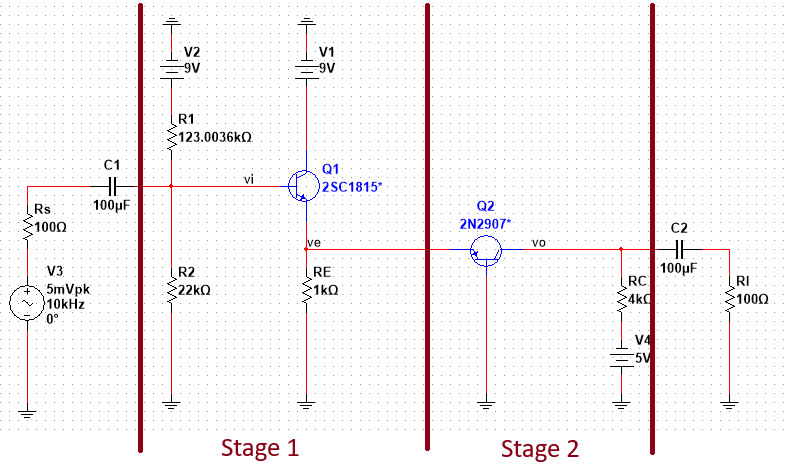
\includegraphics[width=.8\linewidth]{./my-chapters/my-images/Question5/c_machtongquan.png}
\end{figure}

\begin{itemize}[label=-]
	\item Với tầng 1
	
	\begin{figure}[H]
		\centering
		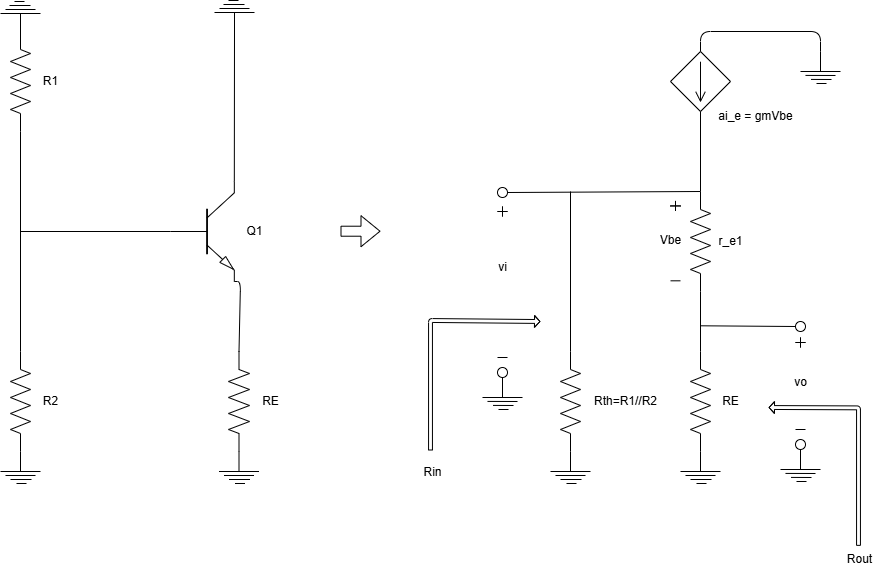
\includegraphics[width=.8\linewidth]{./my-chapters/my-diagrams/Question5/cauc_stage1.png}
	\end{figure}
	
	\begin{itemize}[label=+, leftmargin=2cm]
		\item $r_{e1} = \dfrac{V_{T}}{I_{E1}} = 18.0560\,\Omega$
		\item $r_{\pi1} = \beta\dfrac{V_{T}}{I_{C1}} = 1.8240\,\text{k}\Omega$
		\item $g_{m1} = \dfrac{I_{C1}}{V_{T}} = 54.824\,\text{mS}$
	\end{itemize}
	
	Tính $R_{in1} = \dfrac{v_{i}}{i_{i}}\bigg|_{i_{o} = 0} = R_{th} // (\beta + 1)(r_{e1} + R_{E})$
	
	$\Rightarrow R_{in1} = 15.7954\,\text{k}\Omega$
	
	Tính $R_{out1} = \dfrac{v_{o}}{i_{o}}\bigg|_{v_{i} = 0} = r_{e1} // R_{E}$
	
	$\Rightarrow R_{out1} = 17.7358\,\Omega$
	
	Tín $A_{vo1} = \dfrac{vo}{vi}\bigg|_{R_{L} = \infty} = \dfrac{R_{E}}{R_{E} + r_{e1}}$
	
	$\Rightarrow A_{vo1} = 0.9823\,\text{V/V}$
	\item Với tầng 2
	
	\begin{figure}[H]
		\centering
		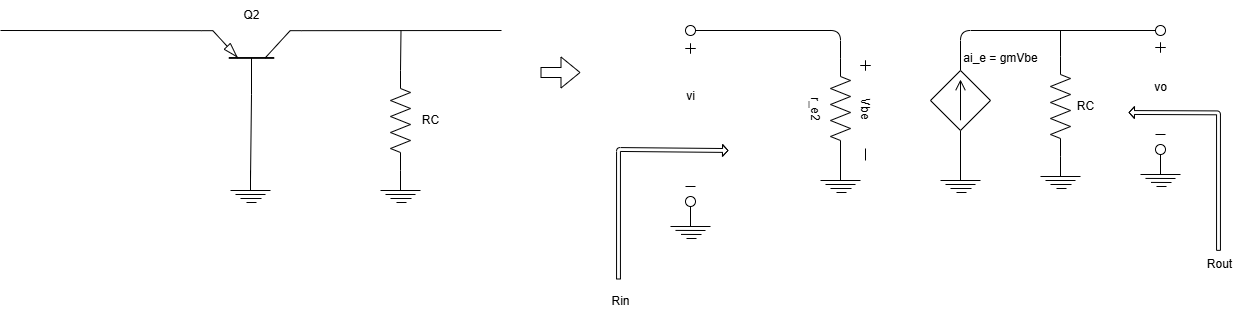
\includegraphics[width=.8\linewidth]{./my-chapters/my-diagrams/Question5/cauc_stagte2.png}
	\end{figure}
	
	\begin{itemize}[label=+, leftmargin=2cm]
		\item $r_{e2} = \dfrac{V_{T}}{I_{E2}} = 33.6585\,\Omega$
		\item $r_{\pi2} = \beta\dfrac{V_{T}}{I_{C2}} = 2.7196\,\text{k}\Omega$
		\item $g_{m2} = \dfrac{I_{C1}}{V_{T}} = 29.416\,\text{mS}$
	\end{itemize}
	
	Tính $R_{in2} = \dfrac{v_{i}}{i_{i}}\bigg|_{i_{o} = 0} = r_{e2}$
	
	$\Rightarrow R_{in2} = 33.6585\,\Omega$
	
	Tính $R_{out2} = \dfrac{v_{o}}{i_{o}}\bigg|_{v_{i} = 0} = R_{C}$
	
	$\Rightarrow R_{out2} = 4\,\text{k}\Omega$
	
	Tín $A_{vo2} = \dfrac{vo}{vi}\bigg|_{R_{L} = \infty} = g_{m2} R_{C}$
	
	$\Rightarrow A_{vo2} = 117.664\,\text{V/V}$
\end{itemize}

Sau khi tính các giá trị của các tầng, ta có mô hình tổng quát như sau

\begin{figure}[H]
	\centering
	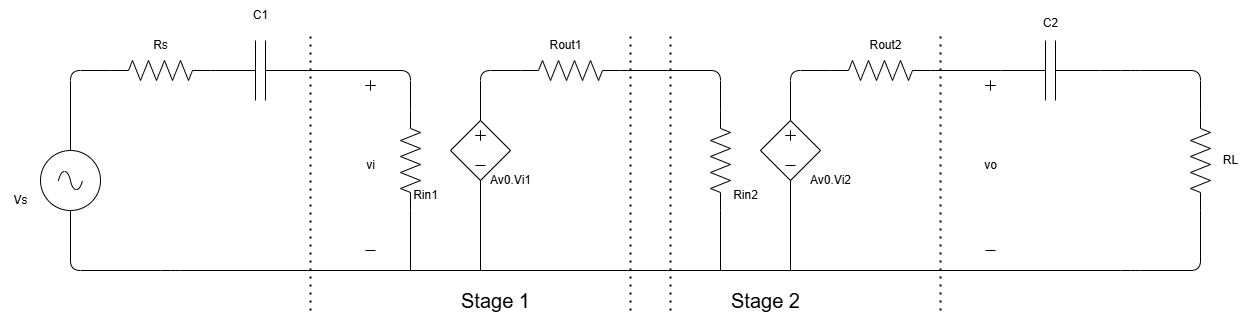
\includegraphics[width=\linewidth]{./my-chapters/my-diagrams/Question5/c_tonghopmach.png}
\end{figure}

\begin{itemize}[label=-]
	\item Xét tụ $C_{1}$:
	\[ \tau_1 = C_{1} \left( R_{s} + R_{in1} \right) \Rightarrow f_{1} = \dfrac{1}{2\pi \tau_1} \]
	\[ \Rightarrow C_{1} = \dfrac{1}{2\pi f_{1} \left( R_{s} + R_{in1} \right)} \]
	
	\item Xét tụ $C_{2}$:
	\[ \tau_{2} = C_{2} \left( R_{out2} + R_{L}\right) \Rightarrow f_{2} = \dfrac{1}{2\pi \tau_{2}}\]
	\[ \Rightarrow C_{2} = \dfrac{1}{2\pi f_{2} \left( R_{out2} + R_{L}\right)}\]
\end{itemize}

Chọn $f_{1} = 200\,\textsf{Hz} = f_{L}$, và cho $f_{2} = \dfrac{f_{1}}{10} = 20\,\textsf{Hz}$

$\Rightarrow$ \finalresult{C_{1} \approx 50.0632 n\,\textsf{F}}.

$\Rightarrow$ \finalresult{C_{2} \approx 1.9409 \,\mu\textsf{F}}.

\begin{figure}[H]
	\centering
	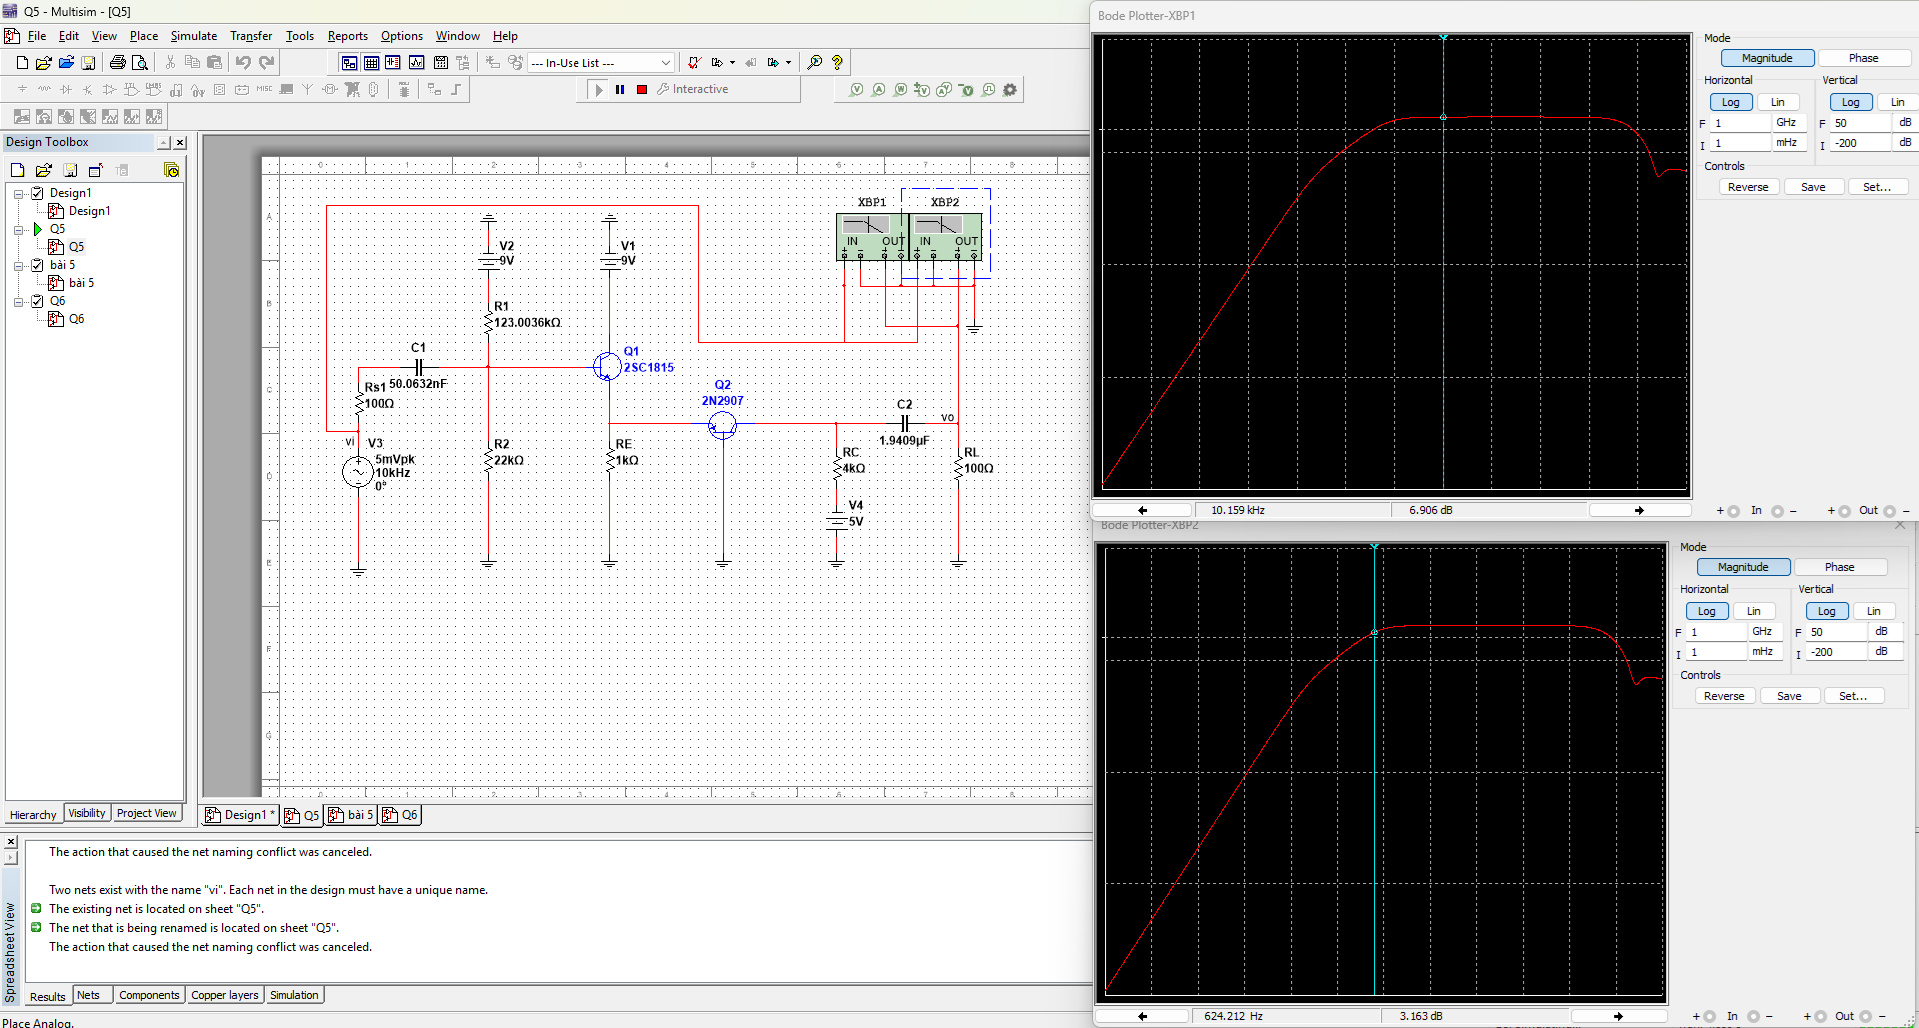
\includegraphics[width=\linewidth]{./my-chapters/my-images/Question5/c_do_bode_socap.png}
	\caption{Ta thấy tại điểm cắt $-3dB$ ta có $f_{L} \approx 624.212\,\textsf{Hz}$.}
\end{figure}

\begin{figure}[H]
	\centering
	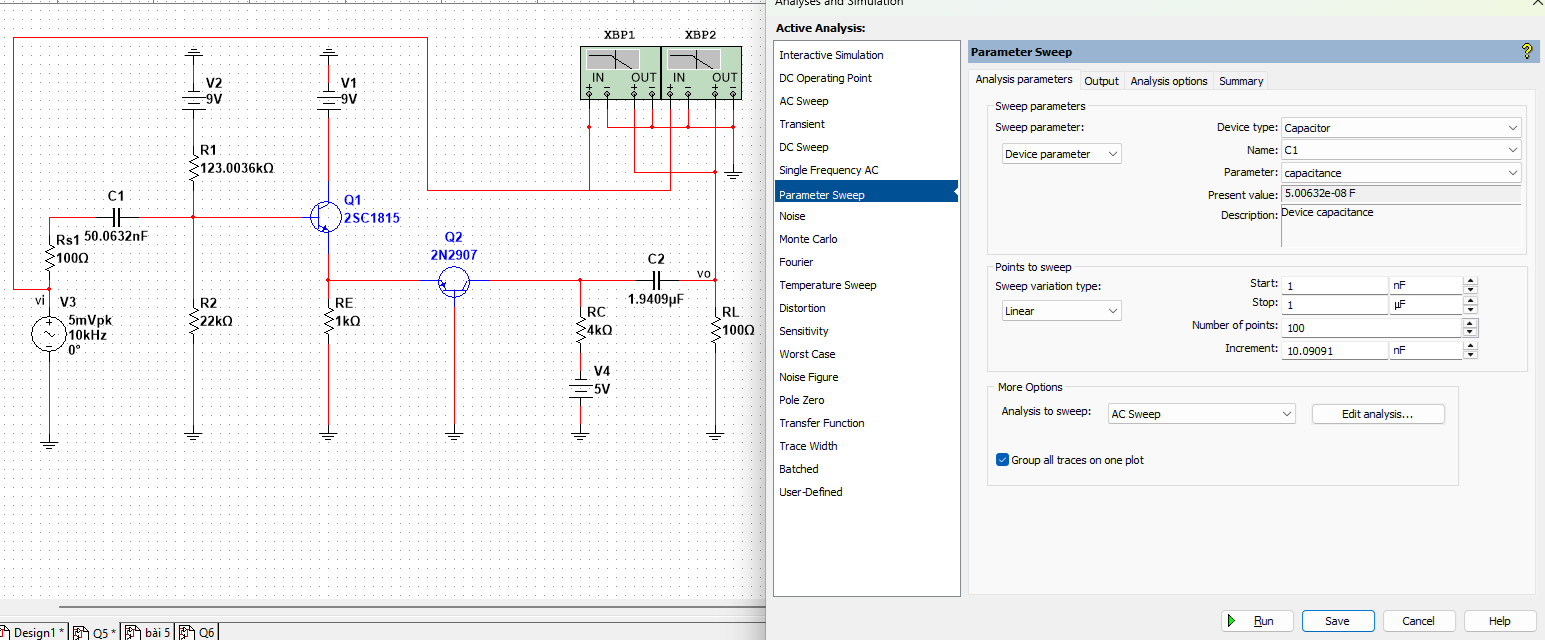
\includegraphics[width=\linewidth]{./my-chapters/my-images/Question5/c_sweep.png}
	\caption{Tiến hành sweep giá trị $C1$ để tìm điểm hợp lý.}
\end{figure}

\begin{figure}[H]
	\centering
	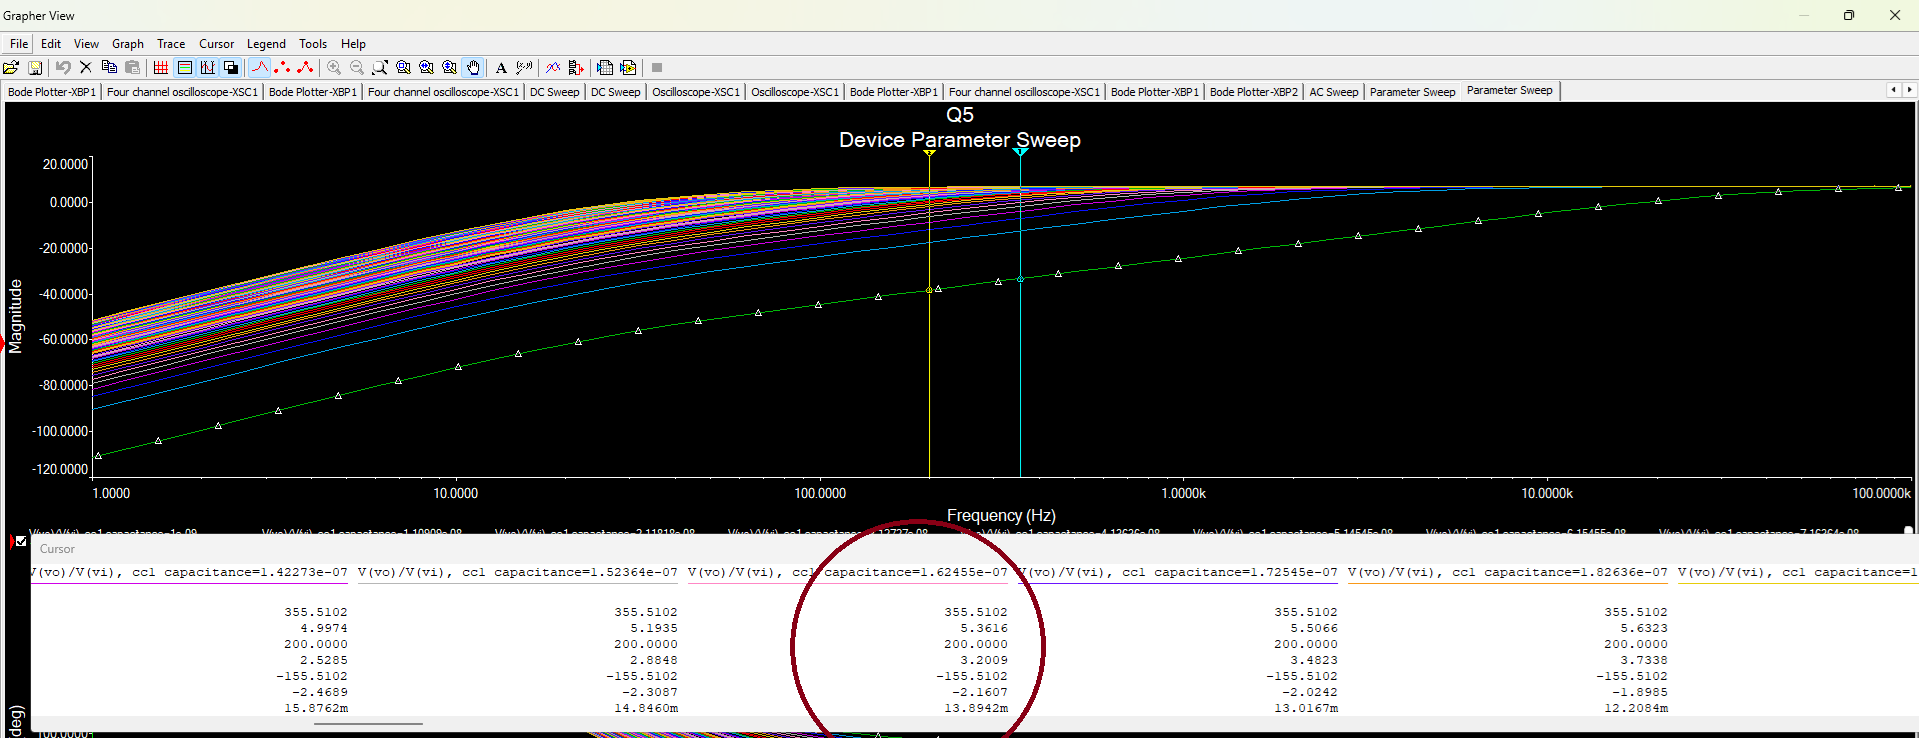
\includegraphics[width=\linewidth]{./my-chapters/my-images/Question5/c_sweep_c.png}
	\caption{Chọn điểm $-3dB$ so với giá trị $G_{v}$ của mạch.}
\end{figure}

Từ ảnh trên ta chọn được \finalresult{C_{1} \approx 162.46 \,\textsf{nF}}.

Tiến hành chạy lại để kiểm tra kết quả cuối cùng

\begin{figure}[H]
	\centering
	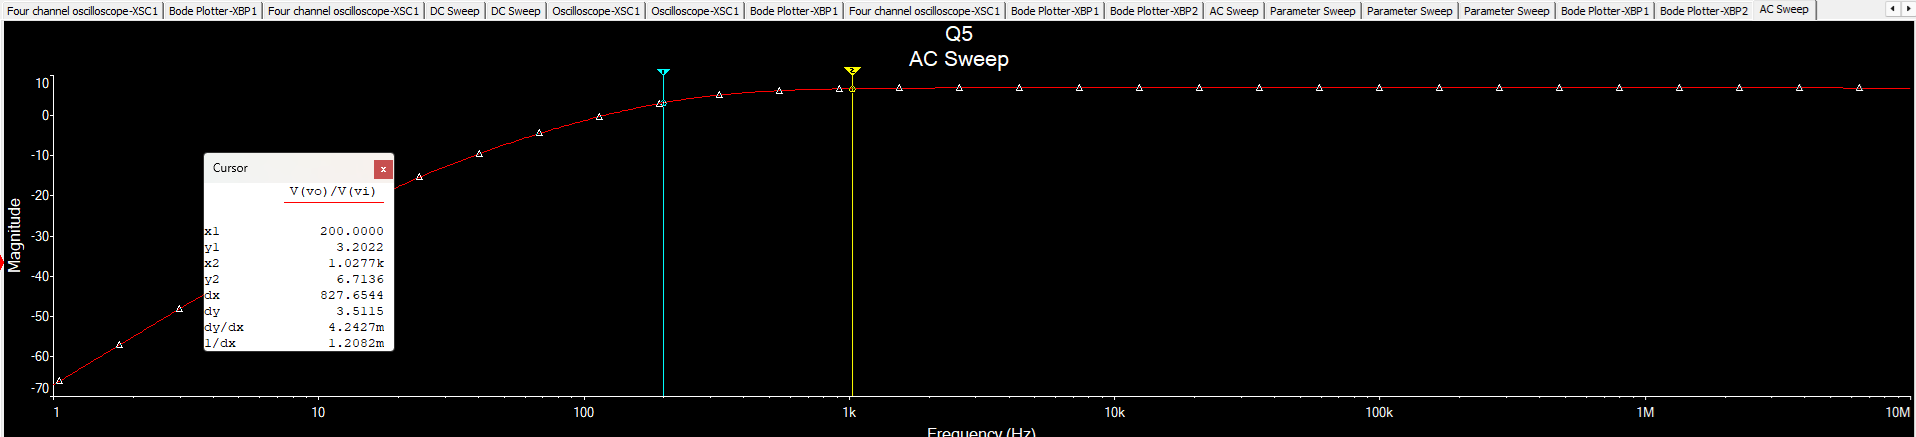
\includegraphics[width=\linewidth]{./my-chapters/my-images/Question5/c_final.png}
	\caption{Sau khi thay đổi $C_{1}$ ta có $f_{L} = 200\,\textsf{Hz}$.}
\end{figure}

\answer{d}{ Đặt vào mạch tín hiệu xoay chiều có biên độ $5\,\text{mV}$ và tần số $10$KHz.  Sử dụng phần mềm mô phỏng, cho biết tín hiệu tại $V_{o1}$ và $V_{o2}$. Giải thích}

\begin{figure}[H]
	\centering
	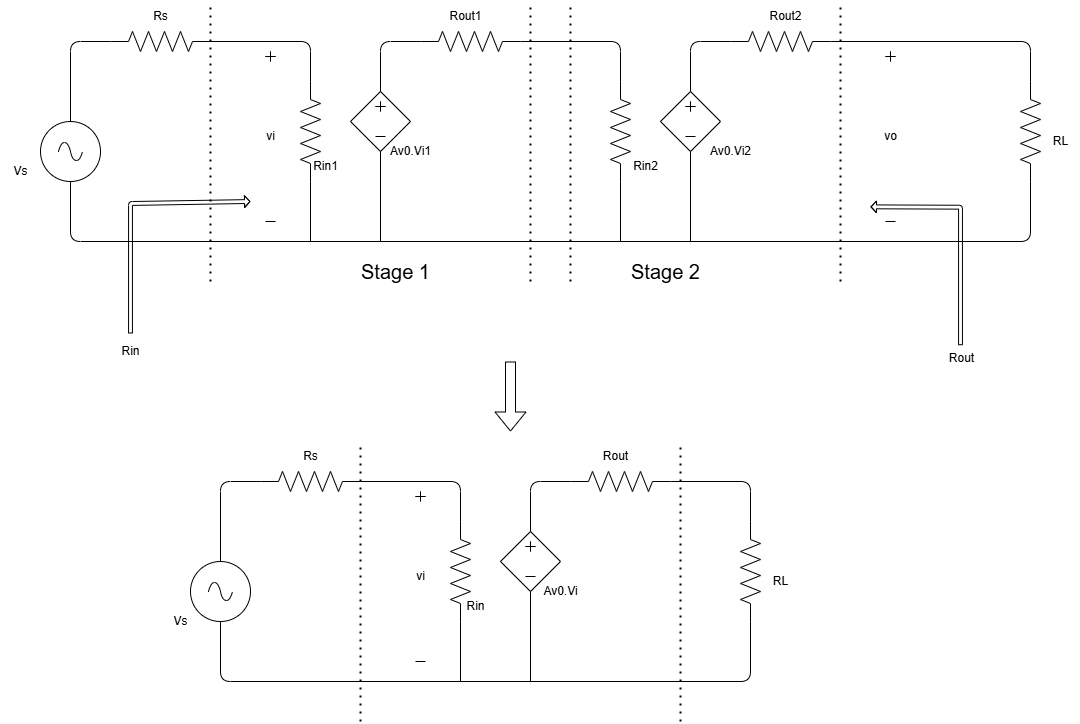
\includegraphics[width=.9\linewidth]{./my-chapters/my-diagrams/Question5/cauc_all_stage.png}
\end{figure}

\begin{itemize}[label=+, leftmargin=2cm]
	\item $A_{vo} = A_{vo2}\dfrac{R_{in2}}{R_{out1} + R_{in2}} A_{vo1} = 75.6951\,\text{V/V}$
	\item $A_{v} = A_{vo} \dfrac{R_{L}}{R_{L} + R_{out2}} = 1.8462\,\text{V/V}$
	\item $G_{v} = \dfrac{R_{s}}{R_{s} + R_{in1}}A_{v} = 1.8346\,\text{V/V} \approx 5.2708dB$
\end{itemize}

\begin{itemize}[label=-]
	\item Tầng 1
	\begin{figure}[H]
		\centering
		\begin{minipage}{.4\linewidth}
			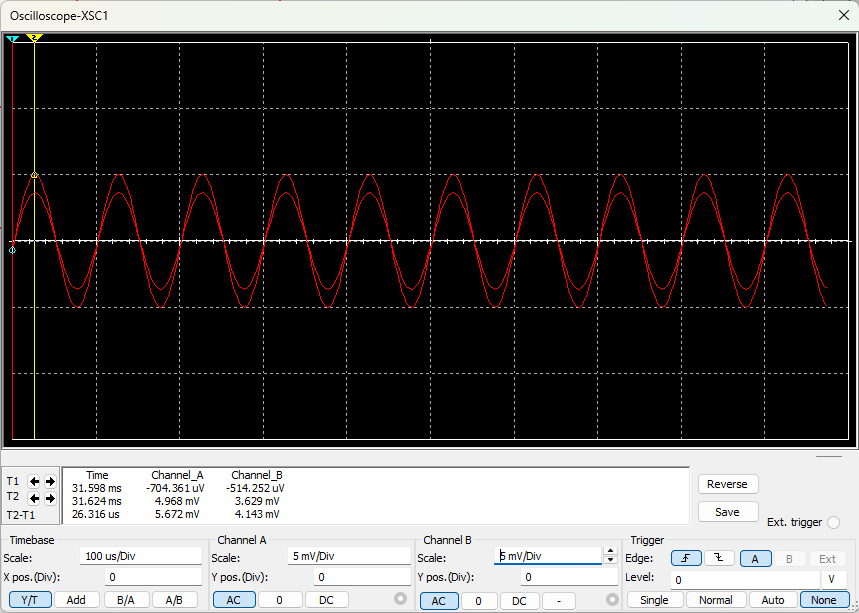
\includegraphics[width=\linewidth]{./my-chapters/my-images/Question5/c_vo1.png}
		\end{minipage}
		\caption{Kết quả khi đo dạng sóng ngỡ ra ở $v_{o1}$.}
	\end{figure}
	
	Vì với $A_{vo1} = 0.9823\,\text{V/V}$ nên tín hiệu ngõ ra có suy giảm một lượng nhỏ so với tín hiệu ngõ vào.
	\item Tầng 2
	\begin{figure}[H]
		\centering
		\begin{minipage}{.4\linewidth}
			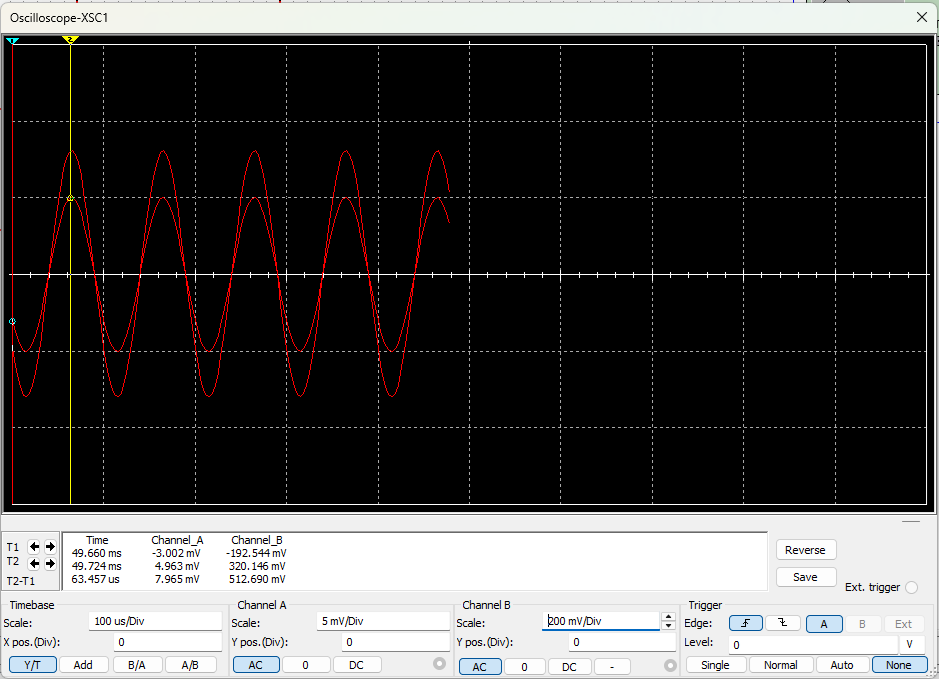
\includegraphics[width=\linewidth]{./my-chapters/my-images/Question5/c_vo2.png}
		\end{minipage}
		\caption{Kết quả khi đo dạng sóng ngỡ ra ở $v_{o2}$.}
	\end{figure}
	
	Vì tới $A_{vo2} = 117.664\,\text{V/V}$ nên tín hiệu ngõ ra ở $v_{o2}$ rất lớn hơn so với tín hiệu ngõ vào.
\end{itemize}

Toàn mạch
\begin{figure}[H]
	\centering
	\begin{minipage}{.4\linewidth}
		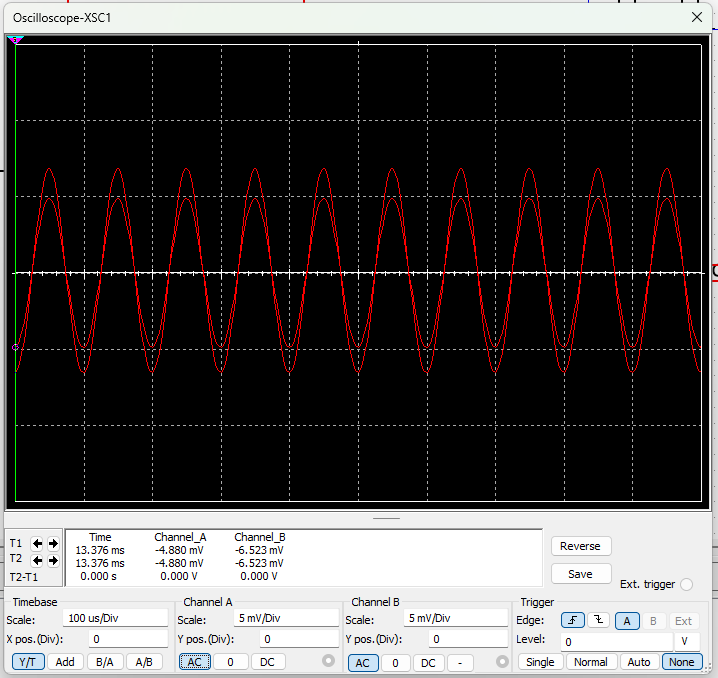
\includegraphics[width=\linewidth]{./my-chapters/my-images/Question5/d_A_Vo.png}
	\end{minipage}
	\begin{minipage}{.4\linewidth}
		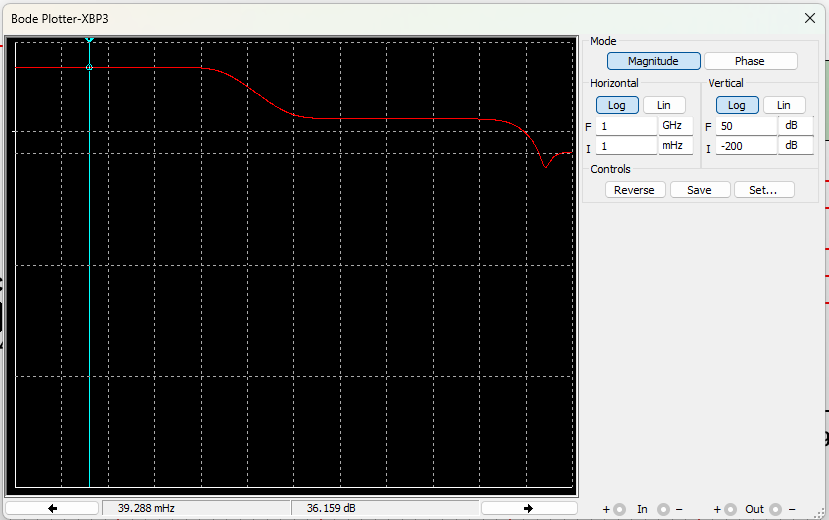
\includegraphics[width=\linewidth]{./my-chapters/my-images/Question5/d_A_vo_ketqua.png}
	\end{minipage}
	\caption{Kết quả khi đo $A_{vo}$ cho toàn mạch.}
\end{figure}
\begin{figure}[H]
	\centering
	\begin{minipage}{.4\linewidth}
		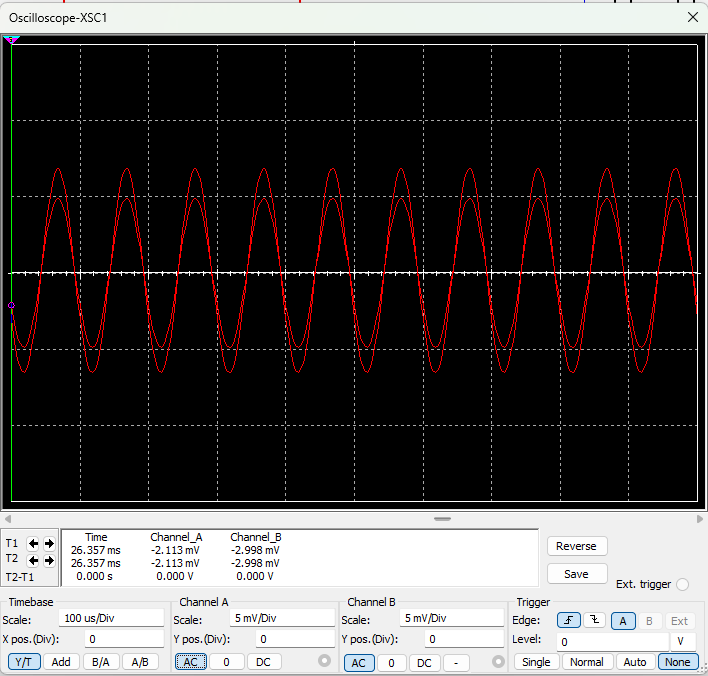
\includegraphics[width=\linewidth]{./my-chapters/my-images/Question5/d_A_V.png}
	\end{minipage}
	\begin{minipage}{.4\linewidth}
		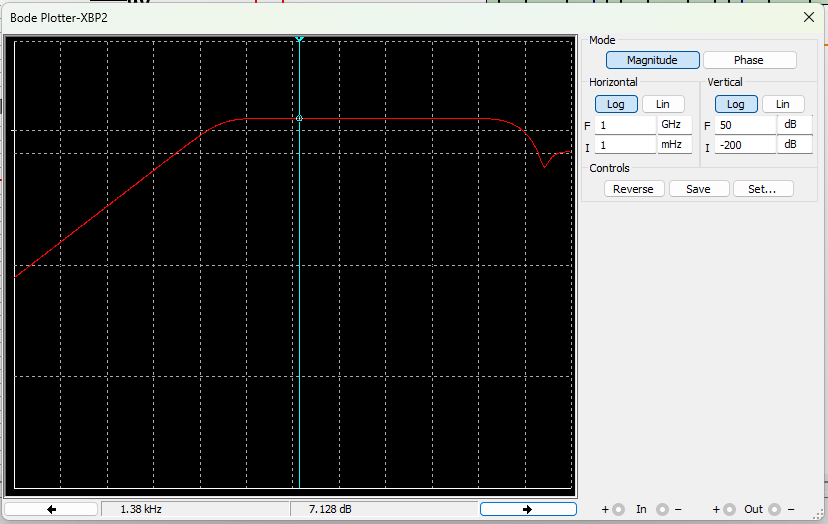
\includegraphics[width=\linewidth]{./my-chapters/my-images/Question5/d_a_v_ketqua.png}
	\end{minipage}
	\caption{Kết quả khi đo $A_{v}$ cho toàn mạch.}
\end{figure}
\begin{figure}[H]
	\centering
	\begin{minipage}{.4\linewidth}
		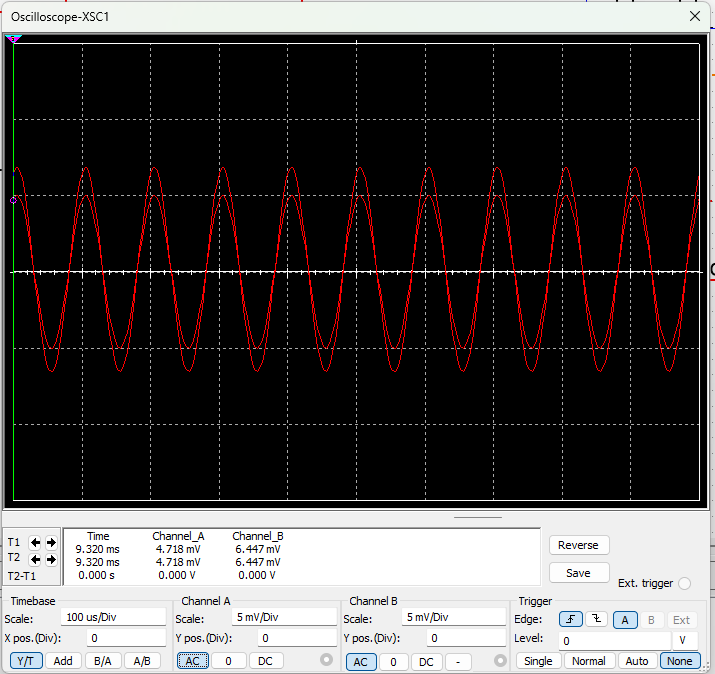
\includegraphics[width=\linewidth]{./my-chapters/my-images/Question5/d_G_V.png}
	\end{minipage}
	\begin{minipage}{.4\linewidth}
		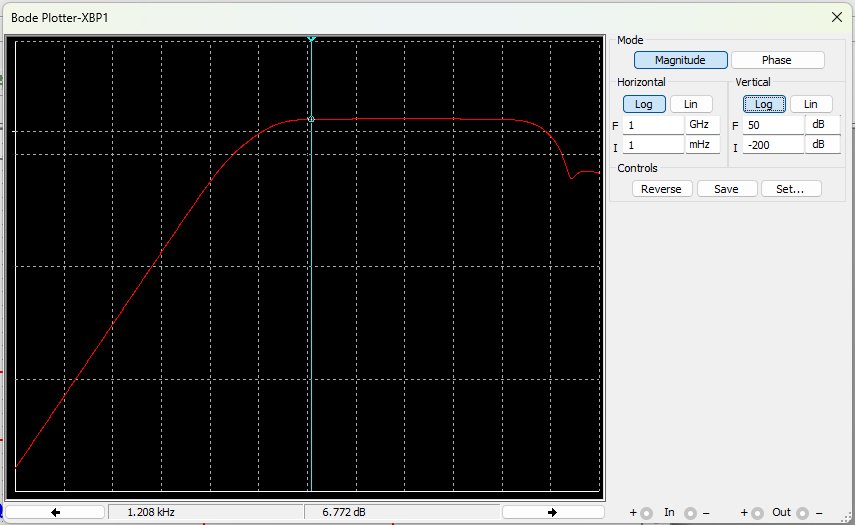
\includegraphics[width=\linewidth]{./my-chapters/my-images/Question5/d_gv_ketqua.png}
	\end{minipage}
	\caption{Kết quả khi đo $G_{v}$ cho toàn mạch.}
\end{figure}